\documentclass{article} % For LaTeX2e
\usepackage{iclr2019_conference,times,enumitem}

% Optional math commands from https://github.com/goodfeli/dlbook_notation.
%%%%% NEW MATH DEFINITIONS %%%%%

\usepackage{amsmath,amsfonts,bm}

% Mark sections of captions for referring to divisions of figures
\newcommand{\figleft}{{\em (Left)}}
\newcommand{\figcenter}{{\em (Center)}}
\newcommand{\figright}{{\em (Right)}}
\newcommand{\figtop}{{\em (Top)}}
\newcommand{\figbottom}{{\em (Bottom)}}
\newcommand{\captiona}{{\em (a)}}
\newcommand{\captionb}{{\em (b)}}
\newcommand{\captionc}{{\em (c)}}
\newcommand{\captiond}{{\em (d)}}

% Highlight a newly defined term
\newcommand{\newterm}[1]{{\bf #1}}


% Figure reference, lower-case.
\def\figref#1{figure~\ref{#1}}
% Figure reference, capital. For start of sentence
\def\Figref#1{Figure~\ref{#1}}
\def\twofigref#1#2{figures \ref{#1} and \ref{#2}}
\def\quadfigref#1#2#3#4{figures \ref{#1}, \ref{#2}, \ref{#3} and \ref{#4}}
% Section reference, lower-case.
\def\secref#1{section~\ref{#1}}
% Section reference, capital.
\def\Secref#1{Section~\ref{#1}}
% Reference to two sections.
\def\twosecrefs#1#2{sections \ref{#1} and \ref{#2}}
% Reference to three sections.
\def\secrefs#1#2#3{sections \ref{#1}, \ref{#2} and \ref{#3}}
% Reference to an equation, lower-case.
\def\eqref#1{equation~\ref{#1}}
% Reference to an equation, upper case
\def\Eqref#1{Equation~\ref{#1}}
% A raw reference to an equation---avoid using if possible
\def\plaineqref#1{\ref{#1}}
% Reference to a chapter, lower-case.
\def\chapref#1{chapter~\ref{#1}}
% Reference to an equation, upper case.
\def\Chapref#1{Chapter~\ref{#1}}
% Reference to a range of chapters
\def\rangechapref#1#2{chapters\ref{#1}--\ref{#2}}
% Reference to an algorithm, lower-case.
\def\algref#1{algorithm~\ref{#1}}
% Reference to an algorithm, upper case.
\def\Algref#1{Algorithm~\ref{#1}}
\def\twoalgref#1#2{algorithms \ref{#1} and \ref{#2}}
\def\Twoalgref#1#2{Algorithms \ref{#1} and \ref{#2}}
% Reference to a part, lower case
\def\partref#1{part~\ref{#1}}
% Reference to a part, upper case
\def\Partref#1{Part~\ref{#1}}
\def\twopartref#1#2{parts \ref{#1} and \ref{#2}}

\def\ceil#1{\lceil #1 \rceil}
\def\floor#1{\lfloor #1 \rfloor}
\def\1{\bm{1}}
\newcommand{\train}{\mathcal{D}}
\newcommand{\valid}{\mathcal{D_{\mathrm{valid}}}}
\newcommand{\test}{\mathcal{D_{\mathrm{test}}}}

\def\eps{{\epsilon}}


% Random variables
\def\reta{{\textnormal{$\eta$}}}
\def\ra{{\textnormal{a}}}
\def\rb{{\textnormal{b}}}
\def\rc{{\textnormal{c}}}
\def\rd{{\textnormal{d}}}
\def\re{{\textnormal{e}}}
\def\rf{{\textnormal{f}}}
\def\rg{{\textnormal{g}}}
\def\rh{{\textnormal{h}}}
\def\ri{{\textnormal{i}}}
\def\rj{{\textnormal{j}}}
\def\rk{{\textnormal{k}}}
\def\rl{{\textnormal{l}}}
% rm is already a command, just don't name any random variables m
\def\rn{{\textnormal{n}}}
\def\ro{{\textnormal{o}}}
\def\rp{{\textnormal{p}}}
\def\rq{{\textnormal{q}}}
\def\rr{{\textnormal{r}}}
\def\rs{{\textnormal{s}}}
\def\rt{{\textnormal{t}}}
\def\ru{{\textnormal{u}}}
\def\rv{{\textnormal{v}}}
\def\rw{{\textnormal{w}}}
\def\rx{{\textnormal{x}}}
\def\ry{{\textnormal{y}}}
\def\rz{{\textnormal{z}}}

% Random vectors
\def\rvepsilon{{\mathbf{\epsilon}}}
\def\rvtheta{{\mathbf{\theta}}}
\def\rva{{\mathbf{a}}}
\def\rvb{{\mathbf{b}}}
\def\rvc{{\mathbf{c}}}
\def\rvd{{\mathbf{d}}}
\def\rve{{\mathbf{e}}}
\def\rvf{{\mathbf{f}}}
\def\rvg{{\mathbf{g}}}
\def\rvh{{\mathbf{h}}}
\def\rvu{{\mathbf{i}}}
\def\rvj{{\mathbf{j}}}
\def\rvk{{\mathbf{k}}}
\def\rvl{{\mathbf{l}}}
\def\rvm{{\mathbf{m}}}
\def\rvn{{\mathbf{n}}}
\def\rvo{{\mathbf{o}}}
\def\rvp{{\mathbf{p}}}
\def\rvq{{\mathbf{q}}}
\def\rvr{{\mathbf{r}}}
\def\rvs{{\mathbf{s}}}
\def\rvt{{\mathbf{t}}}
\def\rvu{{\mathbf{u}}}
\def\rvv{{\mathbf{v}}}
\def\rvw{{\mathbf{w}}}
\def\rvx{{\mathbf{x}}}
\def\rvy{{\mathbf{y}}}
\def\rvz{{\mathbf{z}}}

% Elements of random vectors
\def\erva{{\textnormal{a}}}
\def\ervb{{\textnormal{b}}}
\def\ervc{{\textnormal{c}}}
\def\ervd{{\textnormal{d}}}
\def\erve{{\textnormal{e}}}
\def\ervf{{\textnormal{f}}}
\def\ervg{{\textnormal{g}}}
\def\ervh{{\textnormal{h}}}
\def\ervi{{\textnormal{i}}}
\def\ervj{{\textnormal{j}}}
\def\ervk{{\textnormal{k}}}
\def\ervl{{\textnormal{l}}}
\def\ervm{{\textnormal{m}}}
\def\ervn{{\textnormal{n}}}
\def\ervo{{\textnormal{o}}}
\def\ervp{{\textnormal{p}}}
\def\ervq{{\textnormal{q}}}
\def\ervr{{\textnormal{r}}}
\def\ervs{{\textnormal{s}}}
\def\ervt{{\textnormal{t}}}
\def\ervu{{\textnormal{u}}}
\def\ervv{{\textnormal{v}}}
\def\ervw{{\textnormal{w}}}
\def\ervx{{\textnormal{x}}}
\def\ervy{{\textnormal{y}}}
\def\ervz{{\textnormal{z}}}

% Random matrices
\def\rmA{{\mathbf{A}}}
\def\rmB{{\mathbf{B}}}
\def\rmC{{\mathbf{C}}}
\def\rmD{{\mathbf{D}}}
\def\rmE{{\mathbf{E}}}
\def\rmF{{\mathbf{F}}}
\def\rmG{{\mathbf{G}}}
\def\rmH{{\mathbf{H}}}
\def\rmI{{\mathbf{I}}}
\def\rmJ{{\mathbf{J}}}
\def\rmK{{\mathbf{K}}}
\def\rmL{{\mathbf{L}}}
\def\rmM{{\mathbf{M}}}
\def\rmN{{\mathbf{N}}}
\def\rmO{{\mathbf{O}}}
\def\rmP{{\mathbf{P}}}
\def\rmQ{{\mathbf{Q}}}
\def\rmR{{\mathbf{R}}}
\def\rmS{{\mathbf{S}}}
\def\rmT{{\mathbf{T}}}
\def\rmU{{\mathbf{U}}}
\def\rmV{{\mathbf{V}}}
\def\rmW{{\mathbf{W}}}
\def\rmX{{\mathbf{X}}}
\def\rmY{{\mathbf{Y}}}
\def\rmZ{{\mathbf{Z}}}

% Elements of random matrices
\def\ermA{{\textnormal{A}}}
\def\ermB{{\textnormal{B}}}
\def\ermC{{\textnormal{C}}}
\def\ermD{{\textnormal{D}}}
\def\ermE{{\textnormal{E}}}
\def\ermF{{\textnormal{F}}}
\def\ermG{{\textnormal{G}}}
\def\ermH{{\textnormal{H}}}
\def\ermI{{\textnormal{I}}}
\def\ermJ{{\textnormal{J}}}
\def\ermK{{\textnormal{K}}}
\def\ermL{{\textnormal{L}}}
\def\ermM{{\textnormal{M}}}
\def\ermN{{\textnormal{N}}}
\def\ermO{{\textnormal{O}}}
\def\ermP{{\textnormal{P}}}
\def\ermQ{{\textnormal{Q}}}
\def\ermR{{\textnormal{R}}}
\def\ermS{{\textnormal{S}}}
\def\ermT{{\textnormal{T}}}
\def\ermU{{\textnormal{U}}}
\def\ermV{{\textnormal{V}}}
\def\ermW{{\textnormal{W}}}
\def\ermX{{\textnormal{X}}}
\def\ermY{{\textnormal{Y}}}
\def\ermZ{{\textnormal{Z}}}

% Vectors
\def\vzero{{\bm{0}}}
\def\vone{{\bm{1}}}
\def\vmu{{\bm{\mu}}}
\def\vtheta{{\bm{\theta}}}
\def\va{{\bm{a}}}
\def\vb{{\bm{b}}}
\def\vc{{\bm{c}}}
\def\vd{{\bm{d}}}
\def\ve{{\bm{e}}}
\def\vf{{\bm{f}}}
\def\vg{{\bm{g}}}
\def\vh{{\bm{h}}}
\def\vi{{\bm{i}}}
\def\vj{{\bm{j}}}
\def\vk{{\bm{k}}}
\def\vl{{\bm{l}}}
\def\vm{{\bm{m}}}
\def\vn{{\bm{n}}}
\def\vo{{\bm{o}}}
\def\vp{{\bm{p}}}
\def\vq{{\bm{q}}}
\def\vr{{\bm{r}}}
\def\vs{{\bm{s}}}
\def\vt{{\bm{t}}}
\def\vu{{\bm{u}}}
\def\vv{{\bm{v}}}
\def\vw{{\bm{w}}}
\def\vx{{\bm{x}}}
\def\vy{{\bm{y}}}
\def\vz{{\bm{z}}}

% Elements of vectors
\def\evalpha{{\alpha}}
\def\evbeta{{\beta}}
\def\evepsilon{{\epsilon}}
\def\evlambda{{\lambda}}
\def\evomega{{\omega}}
\def\evmu{{\mu}}
\def\evpsi{{\psi}}
\def\evsigma{{\sigma}}
\def\evtheta{{\theta}}
\def\eva{{a}}
\def\evb{{b}}
\def\evc{{c}}
\def\evd{{d}}
\def\eve{{e}}
\def\evf{{f}}
\def\evg{{g}}
\def\evh{{h}}
\def\evi{{i}}
\def\evj{{j}}
\def\evk{{k}}
\def\evl{{l}}
\def\evm{{m}}
\def\evn{{n}}
\def\evo{{o}}
\def\evp{{p}}
\def\evq{{q}}
\def\evr{{r}}
\def\evs{{s}}
\def\evt{{t}}
\def\evu{{u}}
\def\evv{{v}}
\def\evw{{w}}
\def\evx{{x}}
\def\evy{{y}}
\def\evz{{z}}

% Matrix
\def\mA{{\bm{A}}}
\def\mB{{\bm{B}}}
\def\mC{{\bm{C}}}
\def\mD{{\bm{D}}}
\def\mE{{\bm{E}}}
\def\mF{{\bm{F}}}
\def\mG{{\bm{G}}}
\def\mH{{\bm{H}}}
\def\mI{{\bm{I}}}
\def\mJ{{\bm{J}}}
\def\mK{{\bm{K}}}
\def\mL{{\bm{L}}}
\def\mM{{\bm{M}}}
\def\mN{{\bm{N}}}
\def\mO{{\bm{O}}}
\def\mP{{\bm{P}}}
\def\mQ{{\bm{Q}}}
\def\mR{{\bm{R}}}
\def\mS{{\bm{S}}}
\def\mT{{\bm{T}}}
\def\mU{{\bm{U}}}
\def\mV{{\bm{V}}}
\def\mW{{\bm{W}}}
\def\mX{{\bm{X}}}
\def\mY{{\bm{Y}}}
\def\mZ{{\bm{Z}}}
\def\mBeta{{\bm{\beta}}}
\def\mPhi{{\bm{\Phi}}}
\def\mLambda{{\bm{\Lambda}}}
\def\mSigma{{\bm{\Sigma}}}

% Tensor
\DeclareMathAlphabet{\mathsfit}{\encodingdefault}{\sfdefault}{m}{sl}
\SetMathAlphabet{\mathsfit}{bold}{\encodingdefault}{\sfdefault}{bx}{n}
\newcommand{\tens}[1]{\bm{\mathsfit{#1}}}
\def\tA{{\tens{A}}}
\def\tB{{\tens{B}}}
\def\tC{{\tens{C}}}
\def\tD{{\tens{D}}}
\def\tE{{\tens{E}}}
\def\tF{{\tens{F}}}
\def\tG{{\tens{G}}}
\def\tH{{\tens{H}}}
\def\tI{{\tens{I}}}
\def\tJ{{\tens{J}}}
\def\tK{{\tens{K}}}
\def\tL{{\tens{L}}}
\def\tM{{\tens{M}}}
\def\tN{{\tens{N}}}
\def\tO{{\tens{O}}}
\def\tP{{\tens{P}}}
\def\tQ{{\tens{Q}}}
\def\tR{{\tens{R}}}
\def\tS{{\tens{S}}}
\def\tT{{\tens{T}}}
\def\tU{{\tens{U}}}
\def\tV{{\tens{V}}}
\def\tW{{\tens{W}}}
\def\tX{{\tens{X}}}
\def\tY{{\tens{Y}}}
\def\tZ{{\tens{Z}}}


% Graph
\def\gA{{\mathcal{A}}}
\def\gB{{\mathcal{B}}}
\def\gC{{\mathcal{C}}}
\def\gD{{\mathcal{D}}}
\def\gE{{\mathcal{E}}}
\def\gF{{\mathcal{F}}}
\def\gG{{\mathcal{G}}}
\def\gH{{\mathcal{H}}}
\def\gI{{\mathcal{I}}}
\def\gJ{{\mathcal{J}}}
\def\gK{{\mathcal{K}}}
\def\gL{{\mathcal{L}}}
\def\gM{{\mathcal{M}}}
\def\gN{{\mathcal{N}}}
\def\gO{{\mathcal{O}}}
\def\gP{{\mathcal{P}}}
\def\gQ{{\mathcal{Q}}}
\def\gR{{\mathcal{R}}}
\def\gS{{\mathcal{S}}}
\def\gT{{\mathcal{T}}}
\def\gU{{\mathcal{U}}}
\def\gV{{\mathcal{V}}}
\def\gW{{\mathcal{W}}}
\def\gX{{\mathcal{X}}}
\def\gY{{\mathcal{Y}}}
\def\gZ{{\mathcal{Z}}}

% Sets
\def\sA{{\mathbb{A}}}
\def\sB{{\mathbb{B}}}
\def\sC{{\mathbb{C}}}
\def\sD{{\mathbb{D}}}
% Don't use a set called E, because this would be the same as our symbol
% for expectation.
\def\sF{{\mathbb{F}}}
\def\sG{{\mathbb{G}}}
\def\sH{{\mathbb{H}}}
\def\sI{{\mathbb{I}}}
\def\sJ{{\mathbb{J}}}
\def\sK{{\mathbb{K}}}
\def\sL{{\mathbb{L}}}
\def\sM{{\mathbb{M}}}
\def\sN{{\mathbb{N}}}
\def\sO{{\mathbb{O}}}
\def\sP{{\mathbb{P}}}
\def\sQ{{\mathbb{Q}}}
\def\sR{{\mathbb{R}}}
\def\sS{{\mathbb{S}}}
\def\sT{{\mathbb{T}}}
\def\sU{{\mathbb{U}}}
\def\sV{{\mathbb{V}}}
\def\sW{{\mathbb{W}}}
\def\sX{{\mathbb{X}}}
\def\sY{{\mathbb{Y}}}
\def\sZ{{\mathbb{Z}}}

% Entries of a matrix
\def\emLambda{{\Lambda}}
\def\emA{{A}}
\def\emB{{B}}
\def\emC{{C}}
\def\emD{{D}}
\def\emE{{E}}
\def\emF{{F}}
\def\emG{{G}}
\def\emH{{H}}
\def\emI{{I}}
\def\emJ{{J}}
\def\emK{{K}}
\def\emL{{L}}
\def\emM{{M}}
\def\emN{{N}}
\def\emO{{O}}
\def\emP{{P}}
\def\emQ{{Q}}
\def\emR{{R}}
\def\emS{{S}}
\def\emT{{T}}
\def\emU{{U}}
\def\emV{{V}}
\def\emW{{W}}
\def\emX{{X}}
\def\emY{{Y}}
\def\emZ{{Z}}
\def\emSigma{{\Sigma}}

% entries of a tensor
% Same font as tensor, without \bm wrapper
\newcommand{\etens}[1]{\mathsfit{#1}}
\def\etLambda{{\etens{\Lambda}}}
\def\etA{{\etens{A}}}
\def\etB{{\etens{B}}}
\def\etC{{\etens{C}}}
\def\etD{{\etens{D}}}
\def\etE{{\etens{E}}}
\def\etF{{\etens{F}}}
\def\etG{{\etens{G}}}
\def\etH{{\etens{H}}}
\def\etI{{\etens{I}}}
\def\etJ{{\etens{J}}}
\def\etK{{\etens{K}}}
\def\etL{{\etens{L}}}
\def\etM{{\etens{M}}}
\def\etN{{\etens{N}}}
\def\etO{{\etens{O}}}
\def\etP{{\etens{P}}}
\def\etQ{{\etens{Q}}}
\def\etR{{\etens{R}}}
\def\etS{{\etens{S}}}
\def\etT{{\etens{T}}}
\def\etU{{\etens{U}}}
\def\etV{{\etens{V}}}
\def\etW{{\etens{W}}}
\def\etX{{\etens{X}}}
\def\etY{{\etens{Y}}}
\def\etZ{{\etens{Z}}}

% The true underlying data generating distribution
\newcommand{\pdata}{p_{\rm{data}}}
% The empirical distribution defined by the training set
\newcommand{\ptrain}{\hat{p}_{\rm{data}}}
\newcommand{\Ptrain}{\hat{P}_{\rm{data}}}
% The model distribution
\newcommand{\pmodel}{p_{\rm{model}}}
\newcommand{\Pmodel}{P_{\rm{model}}}
\newcommand{\ptildemodel}{\tilde{p}_{\rm{model}}}
% Stochastic autoencoder distributions
\newcommand{\pencode}{p_{\rm{encoder}}}
\newcommand{\pdecode}{p_{\rm{decoder}}}
\newcommand{\precons}{p_{\rm{reconstruct}}}

\newcommand{\laplace}{\mathrm{Laplace}} % Laplace distribution

\newcommand{\E}{\mathbb{E}}
\newcommand{\Ls}{\mathcal{L}}
\newcommand{\R}{\mathbb{R}}
\newcommand{\emp}{\tilde{p}}
\newcommand{\lr}{\alpha}
\newcommand{\reg}{\lambda}
\newcommand{\rect}{\mathrm{rectifier}}
\newcommand{\softmax}{\mathrm{softmax}}
\newcommand{\sigmoid}{\sigma}
\newcommand{\softplus}{\zeta}
\newcommand{\KL}{D_{\mathrm{KL}}}
\newcommand{\Var}{\mathrm{Var}}
\newcommand{\standarderror}{\mathrm{SE}}
\newcommand{\Cov}{\mathrm{Cov}}
% Wolfram Mathworld says $L^2$ is for function spaces and $\ell^2$ is for vectors
% But then they seem to use $L^2$ for vectors throughout the site, and so does
% wikipedia.
\newcommand{\normlzero}{L^0}
\newcommand{\normlone}{L^1}
\newcommand{\normltwo}{L^2}
\newcommand{\normlp}{L^p}
\newcommand{\normmax}{L^\infty}

\newcommand{\parents}{Pa} % See usage in notation.tex. Chosen to match Daphne's book.

\DeclareMathOperator*{\argmax}{arg\,max}
\DeclareMathOperator*{\argmin}{arg\,min}

\DeclareMathOperator{\sign}{sign}
\DeclareMathOperator{\Tr}{Tr}
\let\ab\allowbreak


\usepackage{hyperref}
\usepackage{url}
\usepackage{graphicx}
\usepackage{caption}
\usepackage{float}
\usepackage{csquotes}


\title{Learning Robust Representations by Projecting Superficial Statistics Out \\ ICLR 2019 Reproducibility Challenge}


\author{Marcin Witkowski \& Łukasz Klasiński \\
Institute of Computer Science \\
University of Wroclaw \\
Wroclaw, Poland \\
\texttt{\{288840,290043\}@uwr.edu.pl} \\
}

\newcommand{\fix}{\marginpar{FIX}}
\newcommand{\new}{\marginpar{NEW}}

\iclrfinalcopy 

\begin{document}

\maketitle

\begin{abstract}
The main goal of reproduced paper is to build a classifier that is not susceptible to covariance shifts, thus making it better in domain generalization. In their work authors introduce new neural building
block - NGLCM, and a method to project out textural information learned by CNN - HEX. In this
paper we tried to reproduce said method and compare results by training model on PACS \citep{Li2017dg}, MNIST and FERG-DB \citep{aneja2016modeling} 
datasets.

\end{abstract}

\section{Method}

\subsection{NGLCM}

NGLCM is a neural block that mimics \textit{gray-level co-occurrence matrix} (GLCM) \citep{glcm}. Main difference is that NGLCM can be trained like any other NN layer during back-propagation, allowing
to tune it's parameters. Thanks to that, this block can extract textural 
information about image but is not capable of extracting semantic information. This is used later to 
unlearn classifier layer from associating textual noises to labels. 

\subsection{HEX}

The main idea of HEX is to project predictions based on all information about data onto subspace that is orthogonal to the ones based on textual-only description of input.
As a result we should obtain predictions which are more independent to covariance shifts, thus more reliable
in domain generalization. It is achieved be using three different outputs:
\begin{align*}
F_A & = f([h(X;\theta), g(X;\phi)];\xi) \\
F_G & = f([\mathbf{0}, g(X;\phi);\xi]) \\
F_P & = f([h(X;\theta), \mathbf{0}];\xi)
\end{align*}
where $F_A$, $F_G$, $F_P$ stands respectively for the results from all representation, only textural representation and raw data.

Projecting $F_A$ onto the subspace that is orthogonal to $F_G$ with
$$F_L = (I - F_G(F_G^T F_G)^{-1} F_G^T) F_A$$
yields $F_L$ for parameter tuning. In testing time $F_P$ is used instead of $F_L$. More information about rationale of this method can be
found in appendix of original paper \citet{wang2018learning}

\pagebreak

\section{Implementation}

Everything was implemented using PyTorch, open-source machine learning library for Python. Since no code was provided with paper,
we had to write everything from scratch. We have performed all tests using Jupyter Notebooks so they are easy to repeat at will.

We have implemented NGLCM block correspondingly to the paper, although we had to guess what direction was used in 
GLCM matrix (we used default of 0), as well as we had to guess MLP layer shape. Another assumption was that the output
of NGLCM is $16\times244$ matrix ($16\times16$ pushed through MLP layer), but we somehow had to make it a vector. To accomplish that we `squashed`
it to $16\cdot244$ length vector to further concatenate it with AlexNet output and pass to HEX's classifier. 

In HEX's case, we calculated $F_A$, $F_G$ and $F_P$ as in paper and finally computed $F_L$. Then results from $F_L$ 
are passed through SoftMax layer.

All of the code is available on our GitHub\footnote{\url{https://github.com/MarWit/nn_project}}

\section{Tests}

\subsection{MNIST tests}

Firstly, we generated 6 datasets, where each of them has 100 images per label, that is 10000 images in total. Subsequent datasets have images rotated by an angle
$\alpha \in \{0^{\circ}, 15^{\circ}, 30^{\circ}, 45^{\circ}, 60^{\circ}, 75^{\circ}\}$, each of them representing one domain.    
All domains but one was used for training and the remaining for testing.

\paragraph{Hyperparameters} 
\begin{itemize}[noitemsep]
    \item optimizer: Adam
    \item learning rate: $10^{-3}$
    \item weight decay: $10^{-3}$
    \item 50 epochs
\end{itemize}

\begin{table}[H]
    \caption{MNIST tests results}
    \centering
    \begin{tabular}{cccc}
        \hline
        Test domain & ADV \citep{wang2018learning} & HEX \citep{wang2018learning} & Our HEX  \\
        \hline
        $\mathcal{M}_{0^{\circ}}$    & 91.1 & 90.1 & 92.3 \\
        $\mathcal{M}_{{15}^{\circ}}$ & 98.2 & 98.9 & 98.7 \\
        $\mathcal{M}_{{30}^{\circ}}$ & 98.6 & 98.9 & 97.1 \\
        $\mathcal{M}_{{45}^{\circ}}$ & 98.7 & 98.8 & 97.9 \\
        $\mathcal{M}_{{60}^{\circ}}$ & 98.4 & 98.3 & 96.5 \\
        $\mathcal{M}_{{75}^{\circ}}$ & 92.0 & 90.0 & 93.1 \\
        \hline
        Avg. & 96.2 & 95.8 & 95.9 \\
        \hline
        
    \end{tabular}
\end{table}

We managed to reproduce results obtained in original paper quite faithfully (Table 3 \citep{wang2018learning}).

\subsection{FERG-DB tests}

\paragraph{Hyperparameters} 
\begin{itemize}[noitemsep]
    \item optimizer: Adam
    \item learning rate: $5\cdot10^{-4}$
    \item 70-100 epochs
\end{itemize}

\pagebreak

As we did not have access to original dataset used in paper, we generated set of 10 datasets based on clean FERG-DB. 
Each of them is created with background correlation $\rho \in[0.0, 0.9]$, which describes how one emotion is correlated with it's background (there are different backgrounds for different emotions).
While we used the same partitioning of data ($50\%$ train, $30\%$ valid, $20\%$ test), each of the datasets had $\approx 10 000$ 
images instead of $50 000$. Sample images from dataset ($\rho=0.8$) are presented below.

\begin{figure}[h]
    \minipage{0.48\textwidth}
    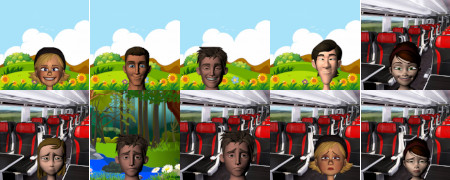
\includegraphics[width=\textwidth]{res/train.jpg}
    \caption*{(a) train set}
    \endminipage\hfill
    \minipage{0.288\textwidth}
    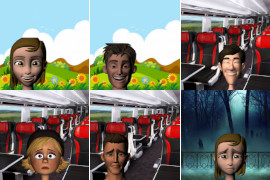
\includegraphics[width=\textwidth]{res/valid.jpg}
    \caption*{(b) validation set}
    \endminipage\hfill
    \minipage{0.192\textwidth}
    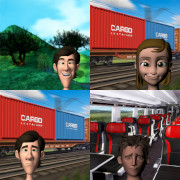
\includegraphics[width=\textwidth]{res/test.jpg}
    \caption*{(c) test set}
    \endminipage\hfill
\end{figure}

We have tested two models on this dataset: normal HEX and modified HEX, where we replaced whole NGLCM block with single 
$224\times16$ MLP layer. In paper, tests with this modification are called `Ablation tests`.

HEX training was converging quickly to $100\%$ accuracy, so we decreased number of epochs to 70 (from 100 in paper) to save time.
We also noticed, that during Ablation tests we sometimes had to rerun training, because model over-fitted on test
data too fast, therefore model could not reach good results on validation set. Also, we were not sure about number of parameters MLP layer should have,
so we picked $224\times16$ since it is a bit less then number of parameters for NGLCM.

\begin{table}[H]
    \caption{FERG-DB tests results}
    \centering
    \begin{tabular}{ccc}
        \hline
        $\rho$ \scriptsize{(background correlation)} & Our HEX with MLP& Our HEX\\
        \hline
        $0.0$ & 98.9 & 99.4 \\
        $0.1$ & 99.2 & 99.6 \\
        $0.2$ & 98.8 & 99.7 \\
        $0.3$ & 98.2 & 99.4 \\
        $0.4$ & 99.0 & 99.1 \\
        $0.5$ & 99.0 & 99.5 \\
        $0.6$ & 98.0 & 99.5 \\
        $0.7$ & 87.2 & 98.4 \\
        $0.8$ & 91.4 & 98.4 \\
        $0.9$ & 49.2 & 91.6 \\
        \hline
        Avg. & 91.9 & 98.5 \\
        \hline
    \end{tabular}
\end{table}
    
HEX with NGLCM is much more stable than bare CNN, yielding similar results
to those from paper (Figure 3.  \citep{wang2018learning}). 
Simple MLP layer isn't capable of removing background noise as well as NGLCM block.

\subsection{PACS tests}
    
Similar to MNIST, we divided images from PACS into 4 domains representing art, cartoon, photo and sketch styled
images. One domain was used for testing and remaining ones for training. We also added random data augmentation (crops and vertical flips) to prevent over-fitting.

\pagebreak

First of all, we trained clean AlexNet.

\paragraph{Hyperparameters Alex} 
\begin{itemize}[noitemsep]
    \item optimizer: Adam
    \item learning rate: $10^{-3}$
    \item weight decay: $0$ or $10^{-2}$
    \item 100 epochs
\end{itemize}

We wanted do get the best results we could, so we used a two step learning. Firstly we have loaded AlexNet pre-trained
on ImageNet dataset (provided by torch library) and trained only classifier. Then, to fine tune the network, we have added
weight decay to optimizer and trained all parameters for additional 50 epochs. We saved model that got best results during
this two stage training and calculated accuracy. 

After getting somehow positive results from AlexNet, we have tested if HEX would perform better or similar using same datasets.

\paragraph{Hyperparameters HEX} 
\begin{itemize}[noitemsep]
    \item optimizer: Adam
    \item learning rate: $10^{-5}$
    \item weight decay: $10^{-5}$
    \item 10+100 epochs
\end{itemize}

Following the paper, we firstly trained classifier layer of pre-trained AlexNet by 10 epochs, then we plugged it into HEX and trained for
additional 100 epochs. At the beginning we had problems with really unstable gradient, so we had to turn learning rate drastically down in 
comparison to the one used in AlexNet. Nonetheless, we didn't really get satisfying results no matter what strategy
we used. At the end, we came to conclusion that in original experiment special PACS heuristics, described in this paper \citep{Li2017dg} was used.
Unfortunately we didn't have enough time to study and replicate such learning method.

\begin{table}[H]
    \caption{PACS domain tests results}
    \centering
    \begin{tabular}{ccccc}
        \hline
        Domain & AlexNet \citep{wang2018learning} & Our AlexNet & HEX \citep{wang2018learning} & Our HEX \\
        \hline
        Art     & 63.3 & 57.2 & 66.8 & 47.6 \\
        Cartoon & 63.1 & 61.3 & 69.7 & 65.0 \\
        Photo   & 87.7 & 81.3 & 87.9 & 53.3 \\
        Sketch  & 54.0 & 62.0 & 56.3 & 57.8 \\
        \hline
        Avg.     & 67.0 & 65.5 & 70.2 & 55.9 \\
        \hline
    \end{tabular}
\end{table}

We have different results in comparison to those from the paper, especially HEX ones. (Table 4 \citep{wang2018learning}). 
Still we think it is strange that under the same conditions HEX performed far worse than AlexNet, which differ from results of \citet{wang2018learning}.

\section{Conclusion}

During reproducibility challenge, we have encountered some minor and major problems.
Paper did not contain most of information about used hyper-parameters and some aspects of described
methods were omitted (ex. used heuristics or how to vectorize output of NGLCM). Overall, we were
able to reproduce results of most of the experiments, besides PACS where we used different heuristic
for fine-tuning CNN.

\pagebreak

\bibliography{iclr2019_conference}
\bibliographystyle{iclr2019_conference}

\end{document}
